%Chapter 2

\renewcommand{\thechapter}{2}

\chapter{Challenges and Motivations}

Many of the world's most influential companies grew from the ashes of the dot-com bubble of the 1990s, which paid for an infrastructure of fiber-optic cables, giant server farms, and research into mobile wireless networks~\cite{casey_blockchain_2018}.
As these companies filled market voids in eCommerce, search, and social networking, they created new database technologies to leverage the potential of underused computational resources and low latency/high bandwidth networks that connected them, eschewing more mature systems that were developed with resource scarcity in mind~\cite{stonebraker_what_2005,stonebraker_mapreduce_2010}.
What followed was the rise and fall of NoSQL data systems, a microcosm of the proceeding era of database research and development~\cite{mohan_history_2013}.
Although there are a lot of facets to the story of NoSQL, what concerns us most is the use of NoSQL to create geographically distributed systems, as these systems paved the way to the large-scale storage systems in use today.

The first phase of distributed NoSQL systems was the creation of highly available, sharded systems intended to meet the demand of increasing numbers of clients.
Commercially, these types of systems include Dynamo~\cite{dynamo} and BigTable~\cite{bigtable}, which in turn spawned open source and academic derivatives such as Cassandra~\cite{cassandra} and HBase~\cite{hbase}.
Although these systems did support large number of accesses, they achieved their availability by relaxing consistency, which many applications found to be intolerable.
The second phase was, therefore, a return to stronger consistency, even at the cost of decreased performance or expensive engineering solutions.
Again, commercial systems led the way with Megastore~\cite{megastore} and Spanner~\cite{spanner} along with academic solutions such as MDCC~\cite{mdcc} and Calvin~\cite{calvindb,calvinfs}.
Part of this realignment was a reconsidering of the base assumption that drove the NoSQL movement expressed in the CAP theorem~\cite{cap}, primarily that the lines between availability, partition tolerance, and consistency may not be as strictly drawn as previously theorized~\cite{hat,consistency_tradeoffs}.
This has led to the beginning of a third phase, the return of SQL, as the lessons learned during the glut of computational resources are applied to more traditional systems.
As before, both commercial systems, such as Aurora~\cite{aurora} and Azure SQL~\cite{azure_sql_database}, and open source systems such as Vitess~\cite{vitess} and CockroachDB~\cite{cockroachdb} are playing an important role in framing the conversation about consistency in this phase.

This brief and limited description of the history of NoSQL distributed systems serves to set the tone for two primary points.
First, designing distributed systems to support a large number of users across large geographies entails a number of challenges and trade-offs due to physical limitations that no single architecture has been able to fully cover.
Second, there exists commercial and practical motivations to build such systems and these motivations have been the impulse toward academic research.
With this backdrop in mind, we explore in this chapter the question of whether a planetary-scale data system is really necessary, and the challenges that we face when designing such systems.

\section{A New Application Development Paradigm}

% Point: global scale applications are the new norm, and they require global scale data storage systems.

The launch of the augmented reality game Pokémon GO in the United States was an unmitigated disaster~\cite{kain_pokemon_2016}.
Due to extremely overloaded servers from the release's extreme popularity, users could not download the game, login, create avatars, or find augmented reality artifacts in their locales.
The company behind the platform, Niantic, scrambled quickly, diverting engineering resources away from their feature roadmap toward improving infrastructure reliability.
The game world was hosted by a suite of Google Cloud services, primarily backed by the Cloud Datastore~\cite{cloud_datastore}, a geographically distributed NoSQL database.
Scaling the application to millions of users therefore involved provisioning extra capacity to the database by increasing the number of shards as well as improving load balancing and autoscaling of application logic run in Kubernetes~\cite{Kubernetes} containers.

Niantic's quick recovery is often hailed as a success story for cloud services and has provided a model for elastic, on demand expansion of computational resources.
A deeper examination, however, shows that Google's global high speed network was at the heart of ensuring that service stayed stable as it expanded ~\cite{stone_bringing_2016}.
The original launch of the game was in 5 countries -- Australia, New Zealand, the United States, the United Kingdom, and Germany; however the success of the game meant worldwide demand, and it was subsequently expanded to over 200 countries starting with Japan~\cite{yamazaki_developer_2016}.
Unlike previous games that were restricted with region locks~\cite{region_locking}, Pokémon GO was a truly international phenomenon and Niantic was determined to allow international interactions in the game's feature set, interaction which relies on Google's unified international architecture and globally distributed databases.

In the brief history of NoSQL that started this chapter, we showed that the growth of database systems distributed across the wide-area started with large internet companies like Yahoo, Google, and Amazon but quickly led to academic investigations.
One reason that the commercial systems enjoyed this academic attention was that at the time, the unique scale of their usage proved the motivation behind their architecture, however their success has meant that these types of scales are no longer limited to huge software systems.
Instead, stories such Niantic's deployment are becoming common and medium to large applications now require developers to increasingly reason about how data is distributed in the wide area, different political regions, and replicated for use around the world.

Consider the following companies and applications from large to small that have international audiences.
Dropbox has users in over 180 countries and is supported in 20 languages, maintaining offices in 12 locations from Herzliya to Sydney \cite{dropbox}.
Slack serves 9 million weekly active users around the world and has 8 offices around the world, prioritizing North America, Europe, and Pacific regions \cite{slack}.
WeWork provides co-working space in 250+ international applications and uses an app to manage global access and membership \cite{wework_global_access}.
Tile has sold 15 million of its RFID trackers worldwide and locates 3 million unique items a day in 230 countries \cite{tile}.
Trello, a project management tool, has been translated into 20 languages and has 250 million world-wide users in every country except Tuvalu, their international rollout focused on marketing and localization \cite{trello}.
Runkeeper~\cite{runkeeper} and DarkSky~\cite{darksky} are iOS and Android apps that have millions of global users and struggled to make their services available in other countries, but benefitted from international app stores.
Signal and Telegraph, encrypted messaging apps have grown primarily in countries at the top of Transparency International's Corruption Perception Index~\cite{signal}.

None of the applications described above necessarily have geography-based requirements in the same way that an augmented reality or airline reservations application might have, just a large number of users who regularly use the app from a variety of geographic locations.
Web developers are increasingly discussing and using container based approaches both for development and small-scale production, web frameworks have built in localization tools that are employed by default, and services are deployed an autoscaling cloud platforms from the start.
The new application development paradigm, even for small applications, is to build with the thought that your application will soon be scaling across the globe.

To address this paradigm, cloud service providers have expanded their offerings to include usage of their distributed data stores to application developers.
The problem is that distributed systems like Dynamo, BigTable, Megastore, and Spanner will all designed for in-house services with a data model that supported replication and eventual consistency, but makes it difficult for developers to reason about behavior, as we will see in the next section.
Not only is there a need for strong consistency semantics, data-location awareness, and geo-replication in distributed data storage systems, there is also the need for a familiar and standardized storage API.

% this explains the shift back to SQL.

\section{Building Geo-Replicated Services}

% Citation for building distributed storage systems?
Given non-geographic requirements for building a distributed system, a common architecture that provides high write throughput with consistent replication

During the first phase of

Paxos as the basis for high performance data store \cite{bolosky_paxos_2011}

What they didn't do and what we do better.

BigTable \& Spanner

S3

Aurora, Cosmos, \& Cockroach DB

Approaches: sharding, independent objects, buckets, slow reads

\begin{figure}
    \begin{center}
        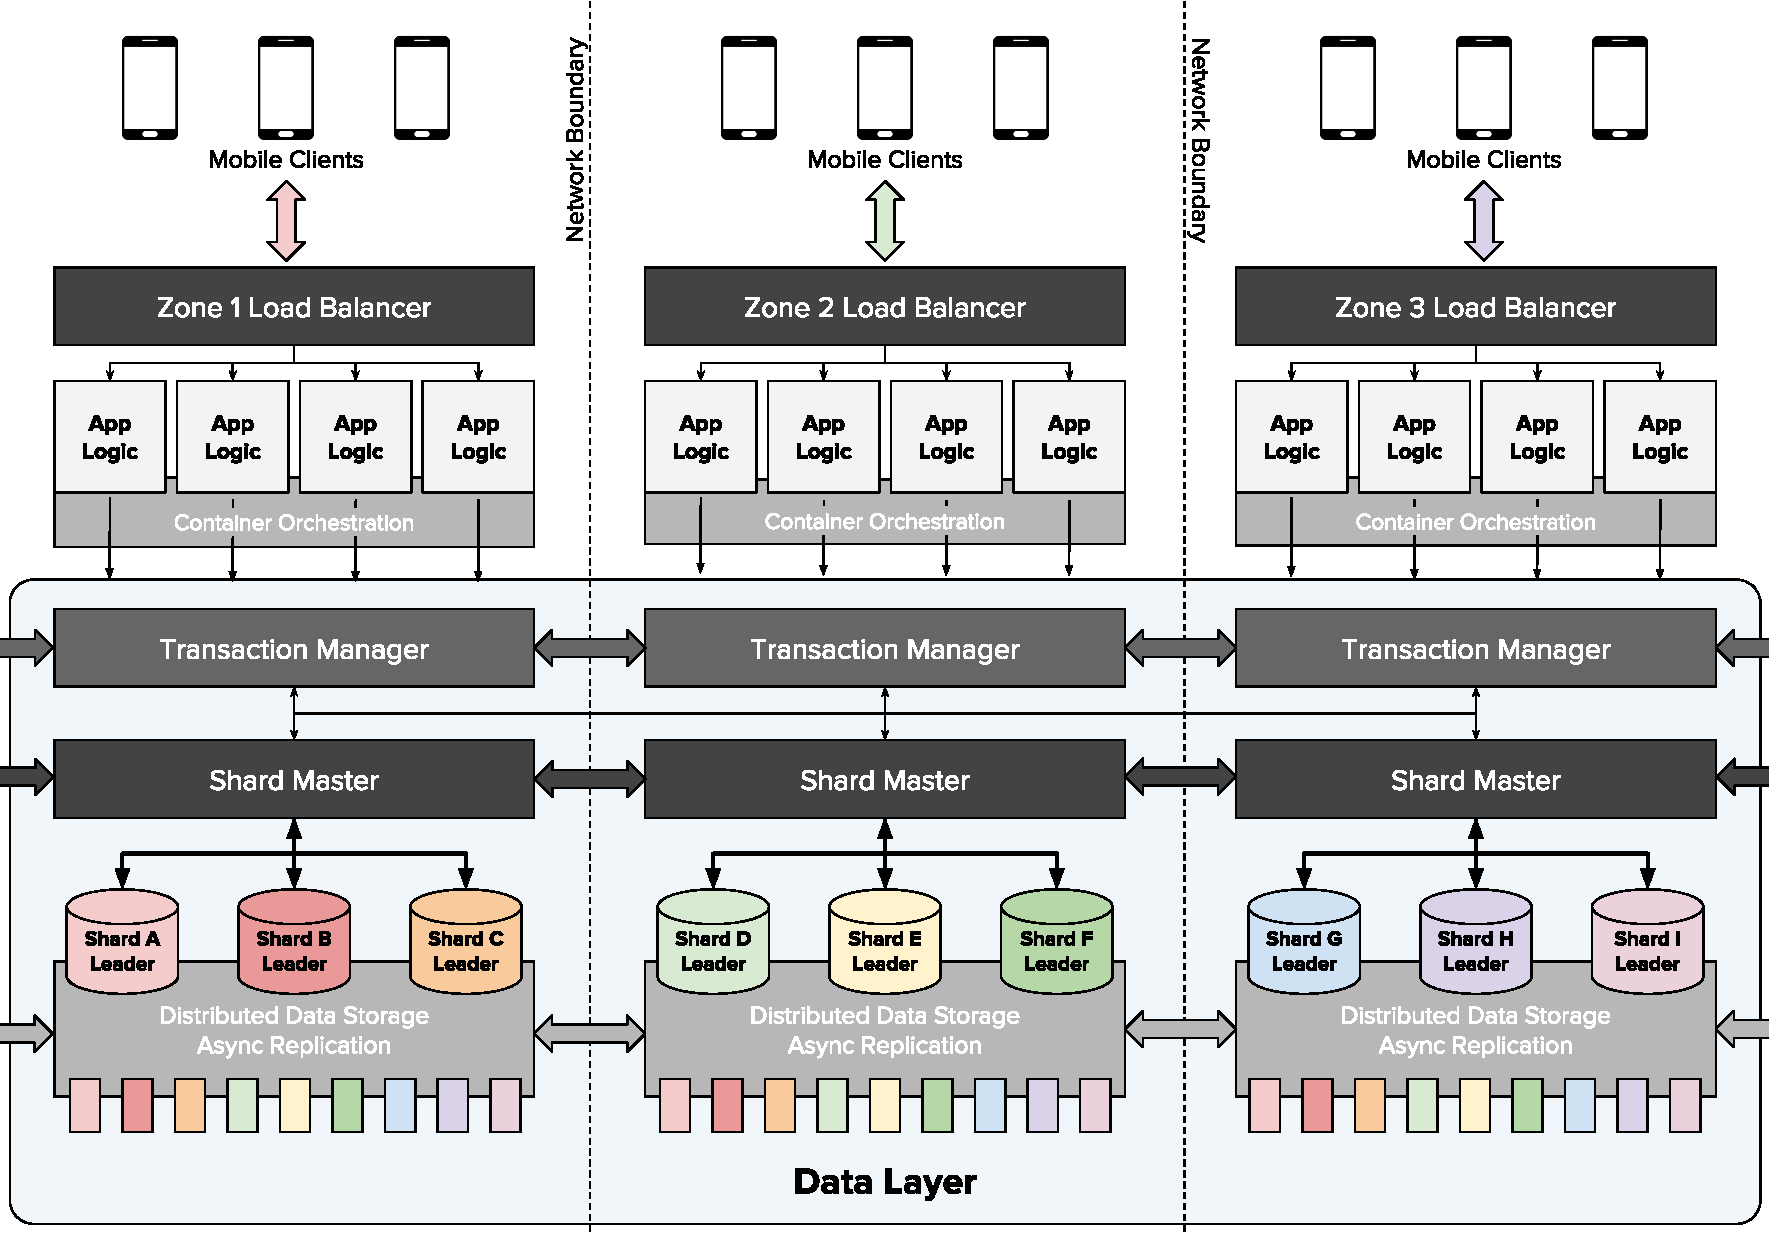
\includegraphics[width=5in]{figures/ch02_distributed_architecture.pdf}
    \end{center}
    \renewcommand{\baselinestretch}{1}
    \small\normalsize

    \begin{quote}
        \caption[Distributed Architectures]{A standard architecture of a distributed application.}
        \label{fig:ch02_distributed_architecture}
    \end{quote}
\end{figure}
\renewcommand{\baselinestretch}{2}
\small\normalsize


\section{Requirements for Data Systems}

Failure is common
    Disk failure/replica failure (ODS)
    Network failure (when repaired, replica comes back online)
    Unreliability: messages have highly variable latency, out of order messaging
    Partitions, part of the system cannot speak to the rest of the system

In geo-systems large latency is not the issue!
    There is a physical limit to message traffic
    Writes must be applied in order, reads can reason about staleness
    Access patterns are also location-dependent

Durability
    Normally 3 disk replication ensures 2 failures
    We need to ensure zone+1 disk failures (re Aurora)
    User-specific data should be accessible everywhere

Fault-Tolerance \& availability
    System should still be available if nodes fail
    Should be available if zones fail (e.g. hurricane or disaster) at higher latency
    System should be available at lower consistency if even one replica is available

Adaptability
    Should respond to changes in user access patterns
    Should be able to add and remove nodes from the system
    Should scale with more regions and more replicas

\section{System Architecture}

Describe the architecture of tier 1: HC, tier 2: Federated Fog

Describe the consistency guarantees we claim

Base application is a key/value store

File-system is built upon the key/value store as an object FS

\begin{figure}
    \begin{center}
        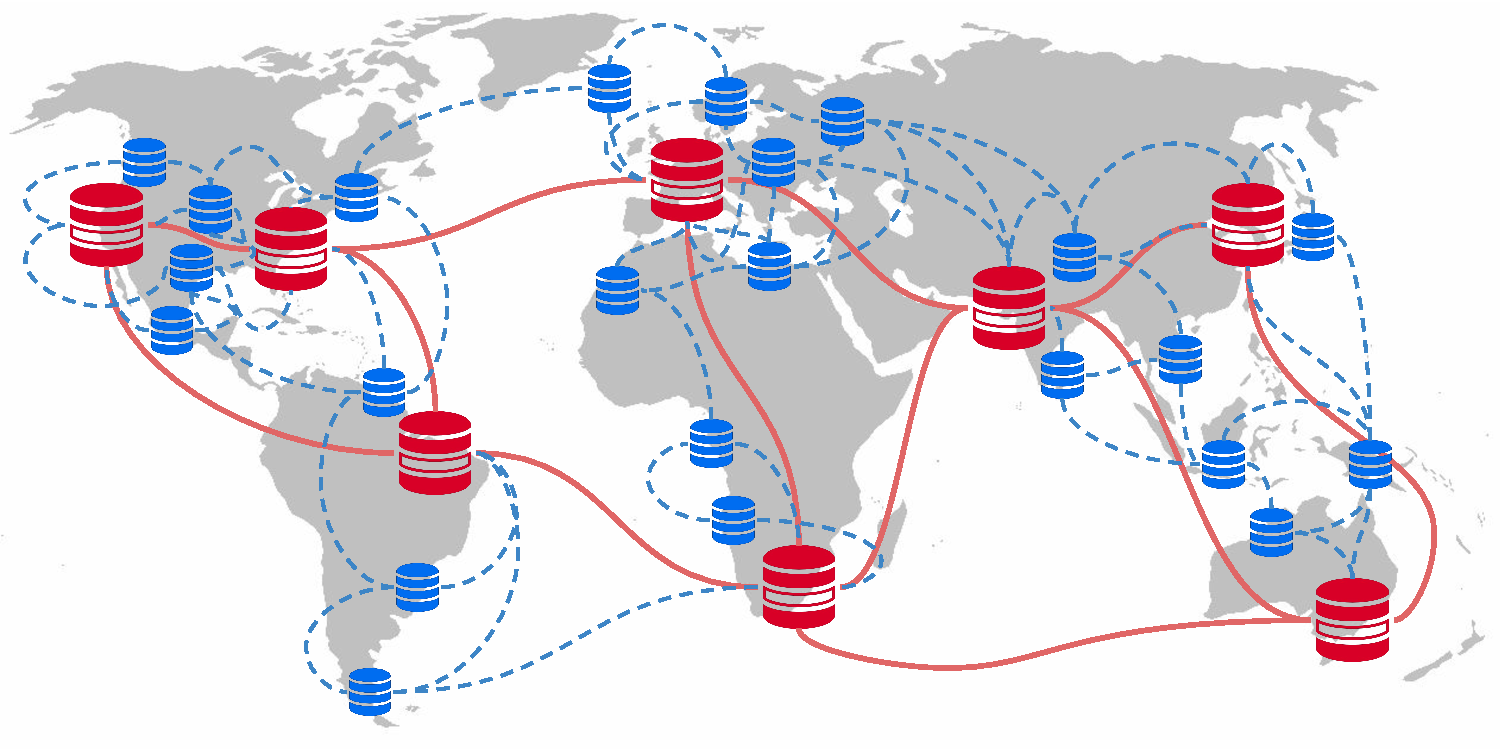
\includegraphics[width=5in]{figures/ch02_global_architecture.pdf}
    \end{center}
    \renewcommand{\baselinestretch}{1}
    \small\normalsize

    \begin{quote}
        \caption[Global Architecture]{A global architecture composed of a core backbone of hierarchical consensus replication (red) and a fog of heterogenous, federated consistency replicas (blue).}
        \label{fig:ch02_global_architecture}
    \end{quote}
\end{figure}
\renewcommand{\baselinestretch}{2}
\small\normalsize

In Figure~\ref{fig:ch02_global_architecture}

\section{Conclusion}

\begin{enumerate}
    \item Global-scale applications are becoming the new norm
    \item Today's globally distributed data systems are high level and require developers to deeply consider consistency and localization semantics.
    \item The challenges are around the physical limitations of geographic networks: the speed of light in this case; e.g. latency and outages.

\end{enumerate}
